\section{Lecture 15: Multirate Signal Processing and Polyphase Representations}
%
\subsection{Changing the Sample Rate By a Non-Integer Factor}
%
Previously, we discussed downsampling and upsampling by an integer rate.
For downsampling by a factor of $M$, we first prefiltered with a low-pass
filter with cutoff frequency $\pi/M$ and gain of $1$ to prevent aliasing,
then downsampled by $M$. For upsampling by a factor of $L$, we padded our
signal with $L-1$ zeroes between each of the original samples, then filtered
with a low-pass filter with cutoff frequency $\pi/L$ and gain of $L$
to interpolate.\\
%
Upsampling or downsampling by integer rates is rather restrictive; there are
many situations where we'd like to use non-integer rates. Consider changing
the sampling rate by the non-integer factor $\tau$, which can be written as
the quotient of two integers, $M/L$. We could in principle make some combination
of upsampling by $L$ and downsampling by $M$ to achieve this. So,
%
\begin{displaymath}
  x[n] \longrightarrow \boxed{\uparrow L}
  \longrightarrow \boxed{H_\mathrm{int}(\omega)}
  \longrightarrow \boxed{H_\mathrm{pre}(\omega)}
  \longrightarrow \boxed{\downarrow M}
  \longrightarrow x_\tau[n] \,.
\end{displaymath}
%
Note that the interpolating filter and prefilter can be condensed into a single
filter; in the frequency domain, we need simply multiply them together, which
results in a single low-pass filter whose cutoff frequency is dictated by
the smallest cutoff frequency of the other two,
%
\begin{displaymath}
  H_\tau(\omega) = H_\mathrm{int}(\omega)H_\mathrm{pre}(\omega)
  \quad \omega_c = \min\left(\frac{\pi}{M},\frac{\pi}{L}\right) \,.
\end{displaymath}
%
If $M>L$, we have a net reduction in sampling rate, meaning $H_\tau(\omega)$
is $H_\mathrm{pre}(\omega)$, and we need to prevent possible aliasing. If
$L>M$, we have a net increase in sampling rate, meaning $H_\tau(\omega)$ is
$H_\mathrm{int}(\omega)$, and we need to interpolate the signal. To give some
numbers, assume $\tau = 1.2$, then we need to upsample by a factor of $5$
and downsample by a factor of $6$, meaning we need to use
$H_\mathrm{pre}(\omega)$.

\subsection{The Noble Identities}
%
This strategy is problematic. Consider $\tau = 1.01$, where $M = 101$ and
$L = 100$, which seems rather wasteful since we're implementing large intermediate
changes in rate to retrieve a signal which is close to the original rate. We then
ask whether this process can be done more efficiently, to which the answer is of
course yes, and is referred to as \textbf{multirate signal processing}.
%
\begin{iden}[\textbf{The Noble Identity for Decimation}]
  The processes
  %
  \begin{displaymath}
    x[n] \longrightarrow \boxed{\downarrow M} \longrightarrow x_a[n]
    \longrightarrow \boxed{H(z)} \longrightarrow y_a[n]
  \end{displaymath}
  %
  and
  %
  \begin{displaymath}
    x[n] \longrightarrow \boxed{H\left(z^M\right)} \longrightarrow x_b[n]
    \longrightarrow \boxed{\downarrow M} \longrightarrow y_b[n]
  \end{displaymath}
  %
  are equivalent.\\

  Let's consider the meaning of $H(z^M)$ for a little insight:
  %
  \begin{displaymath}
    H(z^M) = \infsum{n} h[n]z^{-Mn} = \infsum{k} h[k/M] z^{-k}
    = \mathscr{Z}(h[k/M]) \,,
  \end{displaymath}
  %
  where $h[k/M]$ is a time-expanded version of $h[n]$, i.e. zero-padded with
  $M-1$ zeroes between each sample. Transforming between the $\omega$ and $z$
  domains, we have the relationship
  %
  \begin{displaymath}
    X(\omega) = \left. X(z) \right|_{z = \ex{\im\omega}} \,.
  \end{displaymath}
  %
  Consequently, we can write the expression
  %
  \begin{displaymath}
    X_b(\omega) = H\left(z^M\right)X(\omega) = H\left(\ex{\im\omega M}\right)X(\omega)
    = H(\omega M) X(\omega)
  \end{displaymath}
  %
  since
  %
  \begin{displaymath}
    \left.H\left(z^M\right)\right|_{z=\ex{\im\omega}}
    = \infsum{n} h[n]\ex{-\im\omega nM} = H(\omega M) \,.
  \end{displaymath}
  %
  We saw in the previous lecture that the downsampling block of $X_b(\omega)$ results in
  %
  \begin{displaymath}
    Y_b(\omega) = \frac{1}{M}\sum_{m=0}^{M-1}X\left(\frac{\omega - 2\pi m}{M}\right)
    H(\omega - 2\pi m)
    = H(\omega)\frac{1}{M}\sum_{m=0}^{M-1} X\left(\frac{\omega - 2\pi m}{M}\right) \,,
  \end{displaymath}
  %
  since $H(\omega)$ is $2\pi$-periodic. But this is simply $H(\omega)$ multiplied by
  the result from having first downsampled by $X(\omega)$ by $M$, and consequently we
  have proven that $Y_b(\omega) = Y_a(\omega)$.
\end{iden}
%
\begin{iden}[\textbf{The Noble Identity for Interpolation}]
  The processes
  %
  \begin{displaymath}
    x[n] \longrightarrow \boxed{\uparrow L} \longrightarrow x_a[n]
    \longrightarrow \boxed{H(z)} \longrightarrow y_a[n]
  \end{displaymath}
  %
  and
  %
  \begin{displaymath}
    x[n] \longrightarrow \boxed{H\left(z^L\right)} \longrightarrow x_b[n]
    \longrightarrow \boxed{\uparrow L} \longrightarrow y_b[n]
  \end{displaymath}
  %
  are equivalent.\\

  Recall that upsampling shrinks the spectrum in the frequency domain by a factor
  $L$. Then
  %
  \begin{displaymath}
    Y_a(\omega) = X_a(\omega L) = X(\omega L)H(\omega L) \,,
  \end{displaymath}
  %
  and similarly
  %
  \begin{displaymath}
    X_b(\omega) = X(\omega L) \,,
  \end{displaymath}
  %
  meaning
  %
  \begin{displaymath}
    Y_b(\omega) = X(\omega L)H(\omega L) \,,
  \end{displaymath}
  %
  and we've proven that $Y_a(\omega) = Y_b(\omega)$. This seemingly innocent looking
  interchange has important computational consequences. If we upsample first, we increase
  our signal length by a factor of $L$, most of the elements being zero. This then
  results in a lot of redundant computation by the subsequent filter which has to
  process the signal in serial. In contrast, if we filter first, we have a significantly
  reduced computational overhead, which can later be upsampled.
\end{iden}

\subsection{The Polyphase Decomposition}
%
Consider some signal $h[n]$, an example of which is depicted in pane (a) of
Figure \ref{fig::lecture_15_subphase_filters}. We can think
of this sum as a sum of simpler signals; $h[n]$ is decomposed into a sum of $M$
subsequences $h_k[n]$, defined as follows,
%
\begin{displaymath}
  h_k[n] = \left\{\begin{array}{ccl}
  h[n+k] & &  n\;\mathrm{mod}\;M = 0 \\
  0 & & \mathrm{otherwise}
  \end{array}\right. \,,
\end{displaymath}
%
i.e. the signal is delayed by $k$ units and every $M\th$ element of $h[n]$ is taken, with $M-1$
zeroes padding between these values. This is simplest to understand pictorially;
for $M=3$, pane (b) of Figure \ref{fig::lecture_15_subphase_filters} shows the decomposition.
We see that the original signal is simply the summation of these subsequences,
%
\begin{displaymath}
  h[n] = \sum_{k=0}^{M-1}h_k[n-k] \,.
\end{displaymath}
%
\begin{figure}[H]
  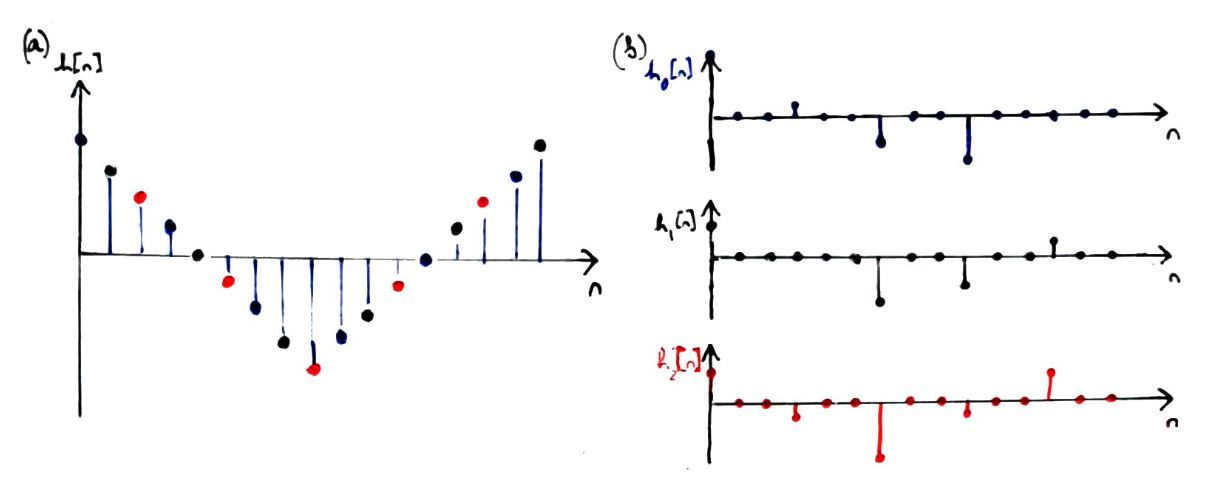
\includegraphics[width=\textwidth]{images/lecture_15_subphase_filters.JPG}
  \caption{Decomposition of a signal, $h[n]$, in pane (a) to a series of 3
    subsequences, $h_0[n], h_1[n]$ and $h_2[n]$, in pane(b), which when shifted and
    added return the original signal.
  }
  \label{fig::lecture_15_subphase_filters}
\end{figure}
%
Let $e_k[n]$ denote a corresponding $h_k[n]$ whose zero-padding has been removed, i.e.
$e_k[n] = h[nM + k] = h_k[nM]$, referred to as the \textbf{subphase filter}, or a
\textbf{polyphase component} of $h[n]$.
Now, consider the Z-transform of $h[n]$ and split it into $M$ distinct sums over
subphase filters,
%
\begin{align*}
  H(z) &= \infsum{k} h[k]z^{-k}
  = \infsum{\ell}h[\ell M]z^{-\ell M} + \infsum{\ell}h[\ell M+1]z^{-(\ell M + 1)} + \hdots \\
  &= \sum_{k=0}^{M-1}\infsum{\ell}h[\ell M + k]z^{-(\ell M + k)}
  = \sum_{k=0}^{M-1}z^{-k}\infsum{\ell}h[\ell M + k]z^{-\ell M} \\
  &= \sum_{k=0}^{M-1}z^{-k} \infsum{\ell}e_k[\ell]z^{-\ell M}
  = \sum_{k=0}^{M-1}z^{-k}\mathscr{E}_k\left(z^M\right) \,,
\end{align*}
%
where $\mathscr{E}_k\left(z^M\right)$ is the Z-transform of the $k\th$ suphase filter
shifted by $M$. Using this as a transfer function,
%
\begin{displaymath}
  Y(z) = H(z)X(z) = \sum_{k=0}^{M-1}z^{-k}\mathscr{E}_k\left(z^M\right)X(z) \,,
\end{displaymath}
%
we see that the $k\th$ term in this summation is the input $X(z)$ delayed by $k$ (since
$X(z)z^{-k} \Longleftrightarrow x[n-k]$), multiplied by the $k\th$ subphase filter expanded
by $M$, $\mathscr{E}\left(z^M\right)$. Each of these terms is then summed to yield the
output, $Y(z)$. This is the \textrm{polyphase realisation} of $H(z)$.\\
%
In an entirely equivalent manner, we can rearrange the above equation so that the
outputs of each polyphase component are delayed. Consider the case where $M=3$:
%
\begin{align*}
  Y(z) &= \mathscr{E}_0\left(z^3\right)X(z) + z^{-1}\mathscr{E}_1\left(z^3\right)X(z)
  + z^{-2}\mathscr{E}_0\left(z^3\right)X(z) \\
  &= \mathscr{E}_0\left(z^3\right)X(z) + z^{-1}\left[
    \mathscr{E}_1\left(z^3\right)X(z) + z^{-1}\left[
      \mathscr{E}_2\left(z^3\right)X(z)
      \right]\right] \,.
\end{align*}
%
This is referred to as the \textbf{transpose polyphase structure}, while the original
is referred to as the \textbf{direct form}. This seemingly innocent looking manipulation
is important when we come to consider upsampling.\\

To offer a little insight, let's consider how we might generate the subphase filter
$\mathscr{E}_k\left(z^M\right)$. We said that this is nothing more than the subphase
filter $\mathscr{E}_k\left(z\right)$ expanded by $M$, i.e. $M-1$ zeroes are placed
between each of the original elements of $\mathscr{E}_k\left(z\right)$, and consequently
it has the same length as the original transfer function before we performed the
polyphase decomposition. To generate $\mathscr{E}_k\left(z\right)$, we need to
implement the following,
%
\begin{displaymath}
  h[n] \longrightarrow \boxed{z^k}
  \longrightarrow \boxed{\downarrow M}
  \longrightarrow e_k[n] \,,
\end{displaymath}
%
so that
$e_0 = \left[\begin{array}{cccc}h[0] & h[M] & h[2M] & \hdots \end{array}\right]^\top$,
$e_1 = \left[\begin{array}{cccc}h[1] & h[M+1] & h[2M+1] & \hdots \end{array}\right]^\top$,
etc. Expanding by $M$ then does nothing more than remove the downsampling by $M$ in
this schematic, such that
%
\begin{displaymath}
  \mathscr{E}_k\left(z^M\right) = H_k(z) \,.
\end{displaymath}

\subsection{Polyphase Downsampling}
%
Now, let's think again about downsampling, where we prefiltered to prevent aliasing
then downsampled the signal,
%
\begin{displaymath}
  x[n] \longrightarrow \boxed{H_{\mathrm{pre}}}
  \longrightarrow \boxed{\downarrow M}
  \longrightarrow y[n] \,.
\end{displaymath}
%
By using the polyphase realisation of our prefilter, we can implement this as depicted in
pane (a) of Figure \ref{fig::lecture_15_polyphase}.
The signal $x[n] = \{x[0], x[1], x[2], \hdots\}$ is passed through
$\mathscr{E}_0\left(z^M\right)$ on the first branch; on the second branch, it
is first delayed by the $z^{-1}$ block yielding $x[n-1] = \{x[-1], x[0], x[1], \hdots\}$,
then passed through $\mathscr{E}_1\left(z^M\right)$, at which point it is summed with the
result from the first branch. This continues up to
$\mathscr{E}_{M-1}\left(z^M\right)$. Once the summation has been completed, the
downsampling $M$ completes the process and we're left with our downsampled signal. The
filtering takes place at a sampling rate of $I_f = I_x$, while at the output after having
downsampled, we have a sampling rate of $I_y = I_x / M$.\\
%
It should be apparent that this is wildly inefficient; the subphase filters
$\mathscr{E}_k\left(z^M\right)$ contain rather a lot of zeroes that don't contribute
anything to the convolution. Consider a prefilter of length 400; convolving a signal
with this requires 400 multiplications and 399 additions per output value. Implementing
this as a polyphase filter bank where we downsample by a factor of 50, all we've
accomplished is 50 subphase filters, each of length 400 and requiring the exact
same computational effort as the original prefilter -- we've just increased the
number of operations by a factor of 50. But now we recall the Noble identity for
decimation,
%
\begin{displaymath}
  x[n] \longrightarrow \boxed{H\left(z^M\right)}
  \longrightarrow \boxed{\downarrow M}
  \longrightarrow y[n]
  \quad\Leftrightarrow\quad
  x[n] \longrightarrow \boxed{\downarrow M}
  \longrightarrow \boxed{H\left(z\right)}
  \longrightarrow y[n]
\end{displaymath}
%
This interchange is depicted in pane (b) of Figure \ref{fig::lecture_15_polyphase}.
Now we can work with the unexpanded subphase filters $\mathscr{E}_k(z)$, thereby
eliminating all of the multiplications by zero in the filtering and each subphase
filter now requires 50 multiplications and 49 additions. Furthermore,
our filtering rate is now $I_f = I_x / M = I_y$, since we downsample before feeding
the input signal into our subphase filters, thus each subphase filter need do $M$
times fewer operations for a signal of some fixed duration. We've thereby reduced
the complexity of our original prefilter by a factor of $M$.\\
%
In terms of implementing this, we can realise the delay line and downsampling as a
commutator which demultiplexes the input line to the different subphase filters with a
frequency of $I_x / M$. This is depicted in pane (a) of Figure
\ref{fig::lecture_15_commutator}, and can be realised in hardware.
%
\begin{figure}[H]
  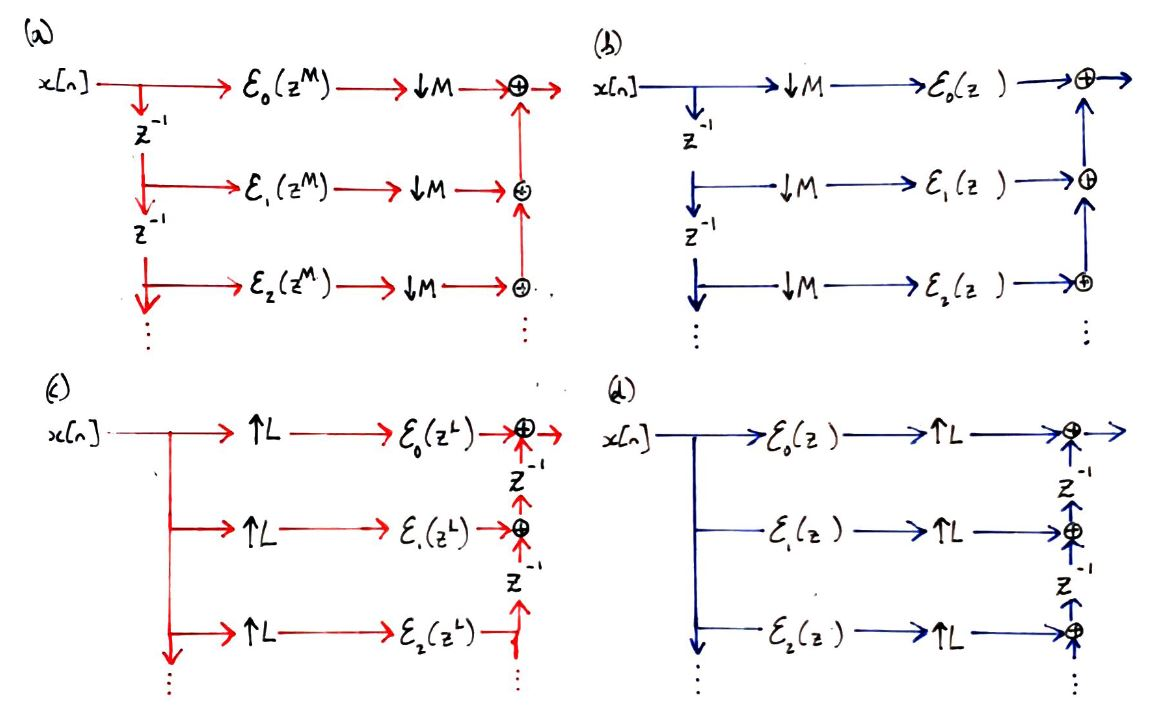
\includegraphics[width=\textwidth]{images/lecture_15_polyphase.JPG}
  \caption{Polyphase implementations of decimation and interpolation. In pane (a),
    the na\"{i}ve decimation filter (using the direct form) is given which filters at a
    rate of $I_x$. By
    invoking the Noble identity for decimation, the structure in pane (b) results
    where each subphase filter operates at a rate of $I_x/M$. In pane (c),
    the na\"{i}ve interpolation filter (using the transpose direct form) is given
    which filters at a rate of $LI_x$. By
    invoking the Noble identity for interpolation, the structure in pane (d) results
    where each subphase filter operates at a rate of $I_x$.
  }
  \label{fig::lecture_15_polyphase}
\end{figure}

\subsection{Polyphase Upsampling}
%
The na\"{i}ve implementation of upsampling has been presented as
%
\begin{displaymath}
  x[n] \longrightarrow \boxed{\uparrow L}
  \longrightarrow \boxed{H_\mathrm{int}}
  \longrightarrow y[n] \,,
\end{displaymath}
%
and the polyphase realisation of the filter $H_\mathrm{int}$ is given in
pane (c) of Figure \ref{fig::lecture_15_polyphase}. As with the decimation, we note that the subphase filters
have a lot of zeroes that contribute nothing to the convolution. Furthermore,
the upsampling components also insert a number of zeroes into the signals
that are fed into the subphase filters. The filtering rate here is $I_f = LI_x$.\\
%
However, we realise that the direct form polyphase structure doesn't work here
since the delay $z^{-k}$ that precedes the subphase filter
$\mathscr{E}_k\left(z^L\right)$ don't commute with the upsampling modules; the
Noble identity for interpolation only allows us to swap the order of subphase filter and
upsampling module. Thankfully, we recall that the transpose polyphase structure allows
us to place the delay lines that accompanies the subphase filters after the filtering.
Now the upsampling modules and subphase filters are next to one another, and the
Noble identity allows us to permute their order,
%
\begin{displaymath}
  x[n] \longrightarrow \boxed{\uparrow L}
  \longrightarrow \boxed{H\left(z^L\right)}
  \longrightarrow y[n]
  \quad\Leftrightarrow\quad
  x[n] \longrightarrow  \boxed{H\left(z\right)}
  \longrightarrow \boxed{\uparrow L}
  \longrightarrow y[n]
\end{displaymath}
%
giving us the realisation depicted in pane (d) of Figure \ref{fig::lecture_15_polyphase}.
The subphase filters no
longer need to be zero-padded with $L-1$ zeroes, and the filtering rate is the same
as the input rate, $I_f = I_x$, in spite of the output signal rate being $I_y = LI_x$.
As with the polyphase decimator, we can turn the delay line and upsampling blocks into
a commutator that multiplexes from the subphase filters to the output line with a rate
of $I_y$. This is depicted in pane (b) of Figure \ref{fig::lecture_15_commutator}.
%
\begin{figure}[H]
  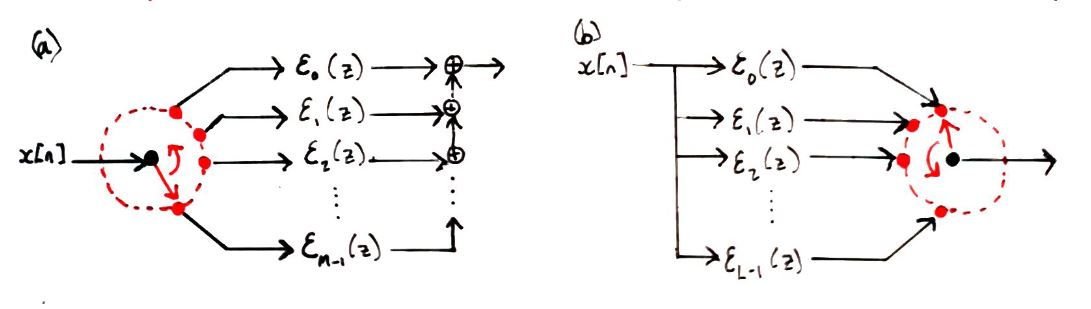
\includegraphics[width=\textwidth]{images/lecture_15_commutator.JPG}
  \caption{Commutator implementations of the polyphase decimation and interpolation.
    In pane (a), the commutator replaces the delay line and downsampling modules,
    and demultiplexes at a rate of $I_x/M$, starting from $\mathscr{E}_{M-1}(z)$ and
    rotating counterclockwise. In pane (b), the commutator replaces the upsampling
    modules and delay line, multiplexing at a rate of $LI_x$ to the output line
    from the subphase filters, starting from $\mathscr{E}_0(z)$ and rotating
    clockwise.
  }
  \label{fig::lecture_15_commutator}
\end{figure}
